\documentclass{article}

%%%%%%%%%%%%%%%%%%%%%%%%%%%%%%%%%
% PACKAGE IMPORTS
%%%%%%%%%%%%%%%%%%%%%%%%%%%%%%%%%


\usepackage[tmargin=2cm,rmargin=1in,lmargin=1in,margin=0.85in,bmargin=2cm,footskip=.2in]{geometry}
\usepackage{amsmath,amsfonts,amsthm,amssymb,mathtools}
% \usepackage[varbb]{newpxmath}
\usepackage{xfrac}
\usepackage[makeroom]{cancel}
\usepackage{mathtools}
\usepackage{bookmark}
\usepackage{enumitem}
\usepackage{hyperref,theoremref}
\hypersetup{
	pdftitle={Assignment},
	colorlinks=true, linkcolor=doc!90,
	bookmarksnumbered=true,
	bookmarksopen=true
}
\usepackage[most,many,breakable]{tcolorbox}
\usepackage{cancel}
\renewcommand{\CancelColor}{\color{red}} % bring in cancel & make it red...
\usepackage{xcolor}
\usepackage{varwidth}
\usepackage{varwidth}
\usepackage{etoolbox}
%\usepackage{authblk}
\usepackage{nameref}
\usepackage{multicol,array}
\usepackage{tikz-cd}
\usepackage[ruled,vlined,linesnumbered]{algorithm2e}
\usepackage{comment} % enables the use of multi-line comments (\ifx \fi) 
\usepackage{import}
\usepackage{xifthen}
\usepackage{pdfpages}
\usepackage{transparent}
\usepackage{pgfplots}
\usepackage{float}

\newcommand\mycommfont[1]{\footnotesize\ttfamily\textcolor{blue}{#1}}
\SetCommentSty{mycommfont}
\newcommand{\incfig}[1]{%
    \def\svgwidth{\columnwidth}
    \import{./figures/}{#1.pdf_tex}
}

\usepackage{tikzsymbols}
\renewcommand\qedsymbol{$\Laughey$}


%\usepackage{import}
%\usepackage{xifthen}
%\usepackage{pdfpages}
%\usepackage{transparent}


%%%%%%%%%%%%%%%%%%%%%%%%%%%%%%
% SELF MADE COLORS
%%%%%%%%%%%%%%%%%%%%%%%%%%%%%%



\definecolor{myg}{RGB}{56, 140, 70}
\definecolor{myb}{RGB}{45, 111, 177}
\definecolor{myr}{RGB}{199, 68, 64}
\definecolor{mytheorembg}{HTML}{F2F2F9}
\definecolor{mytheoremfr}{HTML}{00007B}
\definecolor{mylenmabg}{HTML}{FFFAF8}
\definecolor{mylenmafr}{HTML}{983b0f}
\definecolor{mypropbg}{HTML}{f2fbfc}
\definecolor{mypropfr}{HTML}{191971}
\definecolor{myexamplebg}{HTML}{F2FBF8}
\definecolor{myexamplefr}{HTML}{88D6D1}
\definecolor{myexampleti}{HTML}{2A7F7F}
\definecolor{mydefinitbg}{HTML}{E5E5FF}
\definecolor{mydefinitfr}{HTML}{3F3FA3}
\definecolor{notesgreen}{RGB}{0,162,0}
\definecolor{myp}{RGB}{197, 92, 212}
\definecolor{mygr}{HTML}{2C3338}
\definecolor{myred}{RGB}{127,0,0}
\definecolor{myyellow}{RGB}{169,121,69}
\definecolor{myexercisebg}{HTML}{F2FBF8}
\definecolor{myexercisefg}{HTML}{88D6D1}


%%%%%%%%%%%%%%%%%%%%%%%%%%%%
% TCOLORBOX SETUPS
%%%%%%%%%%%%%%%%%%%%%%%%%%%%

\setlength{\parindent}{1cm}
%================================
% THEOREM BOX
%================================

\tcbuselibrary{theorems,skins,hooks}
\newtcbtheorem[number within=section]{Theorem}{Theorem}
{%
	enhanced,
	breakable,
	colback = mytheorembg,
	frame hidden,
	boxrule = 0sp,
	borderline west = {2pt}{0pt}{mytheoremfr},
	sharp corners,
	detach title,
	before upper = \tcbtitle\par\smallskip,
	coltitle = mytheoremfr,
	fonttitle = \bfseries\sffamily,
	description font = \mdseries,
	separator sign none,
	segmentation style={solid, mytheoremfr},
}
{th}

\tcbuselibrary{theorems,skins,hooks}
\newtcbtheorem[number within=section]{theorem}{Theorem}
{%
	enhanced,
	breakable,
	colback = mytheorembg,
	frame hidden,
	boxrule = 0sp,
	borderline west = {2pt}{0pt}{mytheoremfr},
	sharp corners,
	detach title,
	before upper = \tcbtitle\par\smallskip,
	coltitle = mytheoremfr,
	fonttitle = \bfseries\sffamily,
	description font = \mdseries,
	separator sign none,
	segmentation style={solid, mytheoremfr},
}
{th}


\tcbuselibrary{theorems,skins,hooks}
\newtcolorbox{Theoremcon}
{%
	enhanced
	,breakable
	,colback = mytheorembg
	,frame hidden
	,boxrule = 0sp
	,borderline west = {2pt}{0pt}{mytheoremfr}
	,sharp corners
	,description font = \mdseries
	,separator sign none
}

%================================
% Corollery
%================================
\tcbuselibrary{theorems,skins,hooks}
\newtcbtheorem[number within=section]{Corollary}{Corollary}
{%
	enhanced
	,breakable
	,colback = myp!10
	,frame hidden
	,boxrule = 0sp
	,borderline west = {2pt}{0pt}{myp!85!black}
	,sharp corners
	,detach title
	,before upper = \tcbtitle\par\smallskip
	,coltitle = myp!85!black
	,fonttitle = \bfseries\sffamily
	,description font = \mdseries
	,separator sign none
	,segmentation style={solid, myp!85!black}
}
{th}
\tcbuselibrary{theorems,skins,hooks}
\newtcbtheorem[number within=section]{corollary}{Corollary}
{%
	enhanced
	,breakable
	,colback = myp!10
	,frame hidden
	,boxrule = 0sp
	,borderline west = {2pt}{0pt}{myp!85!black}
	,sharp corners
	,detach title
	,before upper = \tcbtitle\par\smallskip
	,coltitle = myp!85!black
	,fonttitle = \bfseries\sffamily
	,description font = \mdseries
	,separator sign none
	,segmentation style={solid, myp!85!black}
}
{th}


%================================
% LENMA
%================================

\tcbuselibrary{theorems,skins,hooks}
\newtcbtheorem[number within=section]{Lenma}{Lenma}
{%
	enhanced,
	breakable,
	colback = mylenmabg,
	frame hidden,
	boxrule = 0sp,
	borderline west = {2pt}{0pt}{mylenmafr},
	sharp corners,
	detach title,
	before upper = \tcbtitle\par\smallskip,
	coltitle = mylenmafr,
	fonttitle = \bfseries\sffamily,
	description font = \mdseries,
	separator sign none,
	segmentation style={solid, mylenmafr},
}
{th}

\tcbuselibrary{theorems,skins,hooks}
\newtcbtheorem[number within=section]{lenma}{Lenma}
{%
	enhanced,
	breakable,
	colback = mylenmabg,
	frame hidden,
	boxrule = 0sp,
	borderline west = {2pt}{0pt}{mylenmafr},
	sharp corners,
	detach title,
	before upper = \tcbtitle\par\smallskip,
	coltitle = mylenmafr,
	fonttitle = \bfseries\sffamily,
	description font = \mdseries,
	separator sign none,
	segmentation style={solid, mylenmafr},
}
{th}


%================================
% PROPOSITION
%================================

\tcbuselibrary{theorems,skins,hooks}
\newtcbtheorem[number within=section]{Prop}{Proposition}
{%
	enhanced,
	breakable,
	colback = mypropbg,
	frame hidden,
	boxrule = 0sp,
	borderline west = {2pt}{0pt}{mypropfr},
	sharp corners,
	detach title,
	before upper = \tcbtitle\par\smallskip,
	coltitle = mypropfr,
	fonttitle = \bfseries\sffamily,
	description font = \mdseries,
	separator sign none,
	segmentation style={solid, mypropfr},
}
{th}

\tcbuselibrary{theorems,skins,hooks}
\newtcbtheorem[number within=section]{prop}{Proposition}
{%
	enhanced,
	breakable,
	colback = mypropbg,
	frame hidden,
	boxrule = 0sp,
	borderline west = {2pt}{0pt}{mypropfr},
	sharp corners,
	detach title,
	before upper = \tcbtitle\par\smallskip,
	coltitle = mypropfr,
	fonttitle = \bfseries\sffamily,
	description font = \mdseries,
	separator sign none,
	segmentation style={solid, mypropfr},
}
{th}


%================================
% CLAIM
%================================

\tcbuselibrary{theorems,skins,hooks}
\newtcbtheorem[number within=section]{claim}{Claim}
{%
	enhanced
	,breakable
	,colback = myg!10
	,frame hidden
	,boxrule = 0sp
	,borderline west = {2pt}{0pt}{myg}
	,sharp corners
	,detach title
	,before upper = \tcbtitle\par\smallskip
	,coltitle = myg!85!black
	,fonttitle = \bfseries\sffamily
	,description font = \mdseries
	,separator sign none
	,segmentation style={solid, myg!85!black}
}
{th}



%================================
% Exercise
%================================

\tcbuselibrary{theorems,skins,hooks}
\newtcbtheorem[number within=section]{Exercise}{Exercise}
{%
	enhanced,
	breakable,
	colback = myexercisebg,
	frame hidden,
	boxrule = 0sp,
	borderline west = {2pt}{0pt}{myexercisefg},
	sharp corners,
	detach title,
	before upper = \tcbtitle\par\smallskip,
	coltitle = myexercisefg,
	fonttitle = \bfseries\sffamily,
	description font = \mdseries,
	separator sign none,
	segmentation style={solid, myexercisefg},
}
{th}

\tcbuselibrary{theorems,skins,hooks}
\newtcbtheorem[number within=section]{exercise}{Exercise}
{%
	enhanced,
	breakable,
	colback = myexercisebg,
	frame hidden,
	boxrule = 0sp,
	borderline west = {2pt}{0pt}{myexercisefg},
	sharp corners,
	detach title,
	before upper = \tcbtitle\par\smallskip,
	coltitle = myexercisefg,
	fonttitle = \bfseries\sffamily,
	description font = \mdseries,
	separator sign none,
	segmentation style={solid, myexercisefg},
}
{th}

%================================
% EXAMPLE BOX
%================================

\newtcbtheorem[number within=section]{Example}{Example}
{%
	colback = myexamplebg
	,breakable
	,colframe = myexamplefr
	,coltitle = myexampleti
	,boxrule = 1pt
	,sharp corners
	,detach title
	,before upper=\tcbtitle\par\smallskip
	,fonttitle = \bfseries
	,description font = \mdseries
	,separator sign none
	,description delimiters parenthesis
}
{ex}

\newtcbtheorem[number within=section]{example}{Example}
{%
	colback = myexamplebg
	,breakable
	,colframe = myexamplefr
	,coltitle = myexampleti
	,boxrule = 1pt
	,sharp corners
	,detach title
	,before upper=\tcbtitle\par\smallskip
	,fonttitle = \bfseries
	,description font = \mdseries
	,separator sign none
	,description delimiters parenthesis
}
{ex}

%================================
% DEFINITION BOX
%================================

\newtcbtheorem[number within=section]{Definition}{Definition}{enhanced,
	before skip=2mm,after skip=2mm, colback=red!5,colframe=red!80!black,boxrule=0.5mm,
	attach boxed title to top left={xshift=1cm,yshift*=1mm-\tcboxedtitleheight}, varwidth boxed title*=-3cm,
	boxed title style={frame code={
					\path[fill=tcbcolback]
					([yshift=-1mm,xshift=-1mm]frame.north west)
					arc[start angle=0,end angle=180,radius=1mm]
					([yshift=-1mm,xshift=1mm]frame.north east)
					arc[start angle=180,end angle=0,radius=1mm];
					\path[left color=tcbcolback!60!black,right color=tcbcolback!60!black,
						middle color=tcbcolback!80!black]
					([xshift=-2mm]frame.north west) -- ([xshift=2mm]frame.north east)
					[rounded corners=1mm]-- ([xshift=1mm,yshift=-1mm]frame.north east)
					-- (frame.south east) -- (frame.south west)
					-- ([xshift=-1mm,yshift=-1mm]frame.north west)
					[sharp corners]-- cycle;
				},interior engine=empty,
		},
	fonttitle=\bfseries,
	title={#2},#1}{def}
\newtcbtheorem[number within=section]{definition}{Definition}{enhanced,
	before skip=2mm,after skip=2mm, colback=red!5,colframe=red!80!black,boxrule=0.5mm,
	attach boxed title to top left={xshift=1cm,yshift*=1mm-\tcboxedtitleheight}, varwidth boxed title*=-3cm,
	boxed title style={frame code={
					\path[fill=tcbcolback]
					([yshift=-1mm,xshift=-1mm]frame.north west)
					arc[start angle=0,end angle=180,radius=1mm]
					([yshift=-1mm,xshift=1mm]frame.north east)
					arc[start angle=180,end angle=0,radius=1mm];
					\path[left color=tcbcolback!60!black,right color=tcbcolback!60!black,
						middle color=tcbcolback!80!black]
					([xshift=-2mm]frame.north west) -- ([xshift=2mm]frame.north east)
					[rounded corners=1mm]-- ([xshift=1mm,yshift=-1mm]frame.north east)
					-- (frame.south east) -- (frame.south west)
					-- ([xshift=-1mm,yshift=-1mm]frame.north west)
					[sharp corners]-- cycle;
				},interior engine=empty,
		},
	fonttitle=\bfseries,
	title={#2},#1}{def}



%================================
% Solution BOX
%================================

\makeatletter
\newtcbtheorem{question}{Question}{enhanced,
	breakable,
	colback=white,
	colframe=myb!80!black,
	attach boxed title to top left={yshift*=-\tcboxedtitleheight},
	fonttitle=\bfseries,
	title={#2},
	boxed title size=title,
	boxed title style={%
			sharp corners,
			rounded corners=northwest,
			colback=tcbcolframe,
			boxrule=0pt,
		},
	underlay boxed title={%
			\path[fill=tcbcolframe] (title.south west)--(title.south east)
			to[out=0, in=180] ([xshift=5mm]title.east)--
			(title.center-|frame.east)
			[rounded corners=\kvtcb@arc] |-
			(frame.north) -| cycle;
		},
	#1
}{def}
\makeatother

%================================
% SOLUTION BOX
%================================

\makeatletter
\newtcolorbox{solution}{enhanced,
	breakable,
	colback=white,
	colframe=myg!80!black,
	attach boxed title to top left={yshift*=-\tcboxedtitleheight},
	title=Solution,
	boxed title size=title,
	boxed title style={%
			sharp corners,
			rounded corners=northwest,
			colback=tcbcolframe,
			boxrule=0pt,
		},
	underlay boxed title={%
			\path[fill=tcbcolframe] (title.south west)--(title.south east)
			to[out=0, in=180] ([xshift=5mm]title.east)--
			(title.center-|frame.east)
			[rounded corners=\kvtcb@arc] |-
			(frame.north) -| cycle;
		},
}
\makeatother

%================================
% Question BOX
%================================

\makeatletter
\newtcbtheorem{qstion}{Question}{enhanced,
	breakable,
	colback=white,
	colframe=mygr,
	attach boxed title to top left={yshift*=-\tcboxedtitleheight},
	fonttitle=\bfseries,
	title={#2},
	boxed title size=title,
	boxed title style={%
			sharp corners,
			rounded corners=northwest,
			colback=tcbcolframe,
			boxrule=0pt,
		},
	underlay boxed title={%
			\path[fill=tcbcolframe] (title.south west)--(title.south east)
			to[out=0, in=180] ([xshift=5mm]title.east)--
			(title.center-|frame.east)
			[rounded corners=\kvtcb@arc] |-
			(frame.north) -| cycle;
		},
	#1
}{def}
\makeatother

\newtcbtheorem[number within=section]{wconc}{Wrong Concept}{
	breakable,
	enhanced,
	colback=white,
	colframe=myr,
	arc=0pt,
	outer arc=0pt,
	fonttitle=\bfseries\sffamily\large,
	colbacktitle=myr,
	attach boxed title to top left={},
	boxed title style={
			enhanced,
			skin=enhancedfirst jigsaw,
			arc=3pt,
			bottom=0pt,
			interior style={fill=myr}
		},
	#1
}{def}



%================================
% NOTE BOX
%================================

\usetikzlibrary{arrows,calc,shadows.blur}
\tcbuselibrary{skins}
\newtcolorbox{note}[1][]{%
	enhanced jigsaw,
	colback=gray!20!white,%
	colframe=gray!80!black,
	size=small,
	boxrule=1pt,
	title=\textbf{Note:-},
	halign title=flush center,
	coltitle=black,
	breakable,
	drop shadow=black!50!white,
	attach boxed title to top left={xshift=1cm,yshift=-\tcboxedtitleheight/2,yshifttext=-\tcboxedtitleheight/2},
	minipage boxed title=1.5cm,
	boxed title style={%
			colback=white,
			size=fbox,
			boxrule=1pt,
			boxsep=2pt,
			underlay={%
					\coordinate (dotA) at ($(interior.west) + (-0.5pt,0)$);
					\coordinate (dotB) at ($(interior.east) + (0.5pt,0)$);
					\begin{scope}
						\clip (interior.north west) rectangle ([xshift=3ex]interior.east);
						\filldraw [white, blur shadow={shadow opacity=60, shadow yshift=-.75ex}, rounded corners=2pt] (interior.north west) rectangle (interior.south east);
					\end{scope}
					\begin{scope}[gray!80!black]
						\fill (dotA) circle (2pt);
						\fill (dotB) circle (2pt);
					\end{scope}
				},
		},
	#1,
}

%%%%%%%%%%%%%%%%%%%%%%%%%%%%%%
% SELF MADE COMMANDS
%%%%%%%%%%%%%%%%%%%%%%%%%%%%%%


\newcommand{\thm}[2]{\begin{Theorem}{#1}{}#2\end{Theorem}}
\newcommand{\cor}[2]{\begin{Corollary}{#1}{}#2\end{Corollary}}
\newcommand{\mlenma}[2]{\begin{Lenma}{#1}{}#2\end{Lenma}}
\newcommand{\mprop}[2]{\begin{Prop}{#1}{}#2\end{Prop}}
\newcommand{\clm}[3]{\begin{claim}{#1}{#2}#3\end{claim}}
\newcommand{\wc}[2]{\begin{wconc}{#1}{}\setlength{\parindent}{1cm}#2\end{wconc}}
\newcommand{\thmcon}[1]{\begin{Theoremcon}{#1}\end{Theoremcon}}
\newcommand{\ex}[2]{\begin{Example}{#1}{}#2\end{Example}}
\newcommand{\dfn}[2]{\begin{Definition}[colbacktitle=red!75!black]{#1}{}#2\end{Definition}}
\newcommand{\dfnc}[2]{\begin{definition}[colbacktitle=red!75!black]{#1}{}#2\end{definition}}
\newcommand{\qs}[2]{\begin{question}{#1}{}#2\end{question}}
\newcommand{\pf}[2]{\begin{myproof}[#1]#2\end{myproof}}
\newcommand{\nt}[1]{\begin{note}#1\end{note}}

\newcommand*\circled[1]{\tikz[baseline=(char.base)]{
		\node[shape=circle,draw,inner sep=1pt] (char) {#1};}}
\newcommand\getcurrentref[1]{%
	\ifnumequal{\value{#1}}{0}
	{??}
	{\the\value{#1}}%
}
\newcommand{\getCurrentSectionNumber}{\getcurrentref{section}}
\newenvironment{myproof}[1][\proofname]{%
	\proof[\bfseries #1: ]%
}{\endproof}

\newcommand{\mclm}[2]{\begin{myclaim}[#1]#2\end{myclaim}}
\newenvironment{myclaim}[1][\claimname]{\proof[\bfseries #1: ]}{}

\newcounter{mylabelcounter}

\makeatletter
\newcommand{\setword}[2]{%
	\phantomsection
	#1\def\@currentlabel{\unexpanded{#1}}\label{#2}%
}
\makeatother




\tikzset{
	symbol/.style={
			draw=none,
			every to/.append style={
					edge node={node [sloped, allow upside down, auto=false]{$#1$}}}
		}
}


% deliminators
\DeclarePairedDelimiter{\abs}{\lvert}{\rvert}
\DeclarePairedDelimiter{\norm}{\lVert}{\rVert}

\DeclarePairedDelimiter{\ceil}{\lceil}{\rceil}
\DeclarePairedDelimiter{\floor}{\lfloor}{\rfloor}
\DeclarePairedDelimiter{\round}{\lfloor}{\rceil}

\newsavebox\diffdbox
\newcommand{\slantedromand}{{\mathpalette\makesl{d}}}
\newcommand{\makesl}[2]{%
\begingroup
\sbox{\diffdbox}{$\mathsurround=0pt#1\mathrm{#2}$}%
\pdfsave
\pdfsetmatrix{1 0 0.2 1}%
\rlap{\usebox{\diffdbox}}%
\pdfrestore
\hskip\wd\diffdbox
\endgroup
}
\newcommand{\dd}[1][]{\ensuremath{\mathop{}\!\ifstrempty{#1}{%
\slantedromand\@ifnextchar^{\hspace{0.2ex}}{\hspace{0.1ex}}}%
{\slantedromand\hspace{0.2ex}^{#1}}}}
\ProvideDocumentCommand\dv{o m g}{%
  \ensuremath{%
    \IfValueTF{#3}{%
      \IfNoValueTF{#1}{%
        \frac{\dd #2}{\dd #3}%
      }{%
        \frac{\dd^{#1} #2}{\dd #3^{#1}}%
      }%
    }{%
      \IfNoValueTF{#1}{%
        \frac{\dd}{\dd #2}%
      }{%
        \frac{\dd^{#1}}{\dd #2^{#1}}%
      }%
    }%
  }%
}
\providecommand*{\pdv}[3][]{\frac{\partial^{#1}#2}{\partial#3^{#1}}}
%  - others
\DeclareMathOperator{\Lap}{\mathcal{L}}
\DeclareMathOperator{\Var}{Var} % varience
\DeclareMathOperator{\Cov}{Cov} % covarience
\DeclareMathOperator{\E}{E} % expected

% Since the amsthm package isn't loaded

% I prefer the slanted \leq
\let\oldleq\leq % save them in case they're every wanted
\let\oldgeq\geq
\renewcommand{\leq}{\leqslant}
\renewcommand{\geq}{\geqslant}

% % redefine matrix env to allow for alignment, use r as default
% \renewcommand*\env@matrix[1][r]{\hskip -\arraycolsep
%     \let\@ifnextchar\new@ifnextchar
%     \array{*\c@MaxMatrixCols #1}}


%\usepackage{framed}
%\usepackage{titletoc}
%\usepackage{etoolbox}
%\usepackage{lmodern}


%\patchcmd{\tableofcontents}{\contentsname}{\sffamily\contentsname}{}{}

%\renewenvironment{leftbar}
%{\def\FrameCommand{\hspace{6em}%
%		{\color{myyellow}\vrule width 2pt depth 6pt}\hspace{1em}}%
%	\MakeFramed{\parshape 1 0cm \dimexpr\textwidth-6em\relax\FrameRestore}\vskip2pt%
%}
%{\endMakeFramed}

%\titlecontents{chapter}
%[0em]{\vspace*{2\baselineskip}}
%{\parbox{4.5em}{%
%		\hfill\Huge\sffamily\bfseries\color{myred}\thecontentspage}%
%	\vspace*{-2.3\baselineskip}\leftbar\textsc{\small\chaptername~\thecontentslabel}\\\sffamily}
%{}{\endleftbar}
%\titlecontents{section}
%[8.4em]
%{\sffamily\contentslabel{3em}}{}{}
%{\hspace{0.5em}\nobreak\itshape\color{myred}\contentspage}
%\titlecontents{subsection}
%[8.4em]
%{\sffamily\contentslabel{3em}}{}{}  
%{\hspace{0.5em}\nobreak\itshape\color{myred}\contentspage}



%%%%%%%%%%%%%%%%%%%%%%%%%%%%%%%%%%%%%%%%%%%
% TABLE OF CONTENTS
%%%%%%%%%%%%%%%%%%%%%%%%%%%%%%%%%%%%%%%%%%%

% \usepackage{tikz}
% \definecolor{doc}{RGB}{0,60,110}
% \usepackage{titletoc}
% \contentsmargin{0cm}
% % \titlecontents{chapter}[3.7pc]
% {\addvspace{30pt}%
% 	\begin{tikzpicture}[remember picture, overlay]%
% 		\draw[fill=doc!60,draw=doc!60] (-7,-.1) rectangle (-0.9,.5);%
% 		\pgftext[left,x=-3.5cm,y=0.2cm]{\color{white}\Large\sc\bfseries Section\ \thecontentslabel};%
% 	\end{tikzpicture}\color{doc!60}\large\sc\bfseries}%
% {}
% {}
% {\;\titlerule\;\large\sc\bfseries Page \thecontentspage
% 	\begin{tikzpicture}[remember picture, overlay]
% 		\draw[fill=doc!60,draw=doc!60] (2pt,0) rectangle (4,0.1pt);
% 	\end{tikzpicture}}%
% \titlecontents{section}[3.7pc]
% {\addvspace{2pt}}
% {\contentslabel[\thecontentslabel]{2pc}}
% {}
% {\hfill\small \thecontentspage}
% []
% \titlecontents*{subsection}[3.7pc]
% {\addvspace{-1pt}\small}
% {}
% {}
% {\ --- \small\thecontentspage}
% [ \textbullet\ ][]

% \makeatletter
% \renewcommand{\tableofcontents}{%
% 	% \chapter*{%
% 	  \vspace*{-20\p@}%
% 	  \begin{tikzpicture}[remember picture, overlay]%
% 		  \pgftext[right,x=15cm,y=0.2cm]{\color{doc!60}\Huge\sc\bfseries \contentsname};%
% 		  \draw[fill=doc!60,draw=doc!60] (13,-.75) rectangle (20,1);%
% 		  \clip (13,-.75) rectangle (20,1);
% 		  \pgftext[right,x=15cm,y=0.2cm]{\color{white}\Huge\sc\bfseries \contentsname};%
% 	  \end{tikzpicture}}%
% 	\@starttoc{toc}}
% \makeatother

\newcommand{\ub}[1]{\underbar{$#1$}}

\newcommand{\p}[3]{\left( \frac{\partial #1}{\partial #2} \right)_{#3}}

\newcommand{\pop}[2]{\left.\frac{\partial}{\partial #1} \right\vert_{#2}}

\newcommand{\highlight}[2]{\colorbox{#1!20}{$\displaystyle#2$}}

\newcommand{\centmini}[2]{%
	\begin{center}
		\begin{minipage}{#1\linewidth}
			#2
		\end{minipage}
	\end{center}
}

\usepackage{tikz-3dplot}
\usepackage{booktabs}
\usepackage{titling}
\usepackage{fancyhdr}
\usetikzlibrary{patterns}

\pretitle{\vspace{-4em}\begin{flushleft}\LARGE} % Adjust the size and alignment
    \posttitle{\end{flushleft}}
    \preauthor{\begin{flushleft}\large} % Adjust the size and alignment
    \postauthor{\hspace{2em} \large \thedate\end{flushleft}} % Place author and date on the same line
    \predate{} % Remove the default date formatting
    \postdate{} % Remove the default date formatting

\pagestyle{fancy}
\fancyhf{} % Clear all header and footer fields
\fancyfoot[R]{\thepage} % Right-align the page number in the footer
\renewcommand{\headrulewidth}{0pt} % Remove the header rule
\renewcommand{\footrulewidth}{0pt} % Remove the footer rule
    

\geometry{
    top=2cm,    % Top margin
    bottom=3cm, % Bottom margin
    left=2.5cm, % Left margin
    right=2.5cm % Right margin
}
\title{\bfseries CHEG231 Homework 7}
\author{Kyle Wodehouse}
\date{}

\begin{document}
\maketitle
\section*{1.}
\usepgflibrary{patterns}
\begin{center}
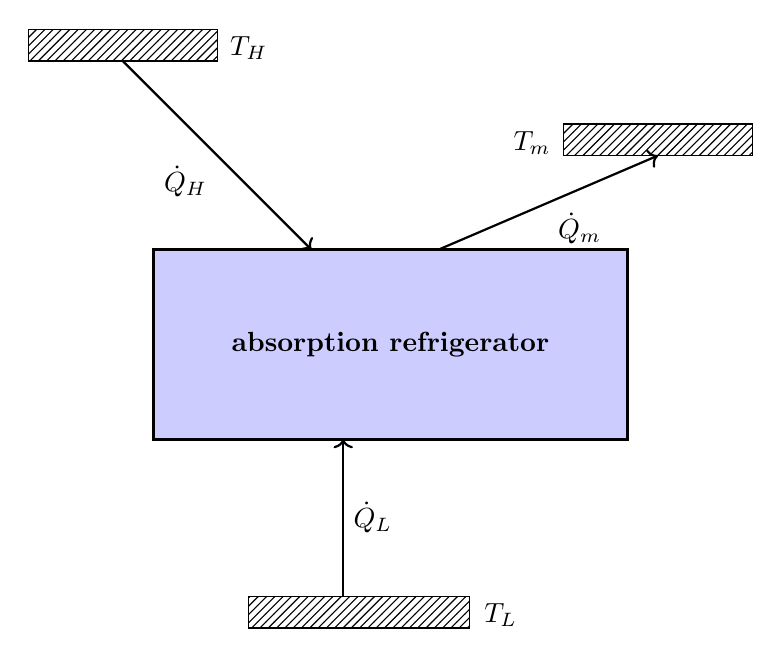
\begin{tikzpicture}[scale=0.8]
    \draw [->, thick]  (5.5, 9.7) -- (8.5, 6.7) node[midway, below left] {$\dot{Q}_{H}$};
    \draw [->, thick]  (10.5, 6.7) -- (14.0, 8.2) node[midway, below right] {$\dot{Q}_{m}$};
    \draw [->, thick]  (9.0, 1.2) -- (9.0, 3.7) node[midway, right] {$\dot{Q}_{L}$};
    \draw[line width=0.5mm] (6.0, 6.7) rectangle (13.5, 3.7);
    \draw[fill=blue!20, draw=black] (6.0, 6.7) rectangle (13.5, 3.7);
    \node at (9.75, 5.2) {\bfseries absorption refrigerator};
    \draw [pattern={north east lines}] (4.0, 10.2) rectangle (7.0, 9.7);
    \node at (7.5, 9.9) {$T_H$};
    \draw [pattern={north east lines}] (12.5, 8.7) rectangle (15.5, 8.2);
    \node at (12.0, 8.4) {$T_m$};
    \draw [pattern={north east lines}] (7.5, 1.2) rectangle (11.0, 0.7);
    \node at (11.5, 0.9) {$T_L$};
\end{tikzpicture}
\end{center}
\subsection*{a}
Let the system be the absorption refrigerator. Assume it operates at steady---state and is reversible. the energy balance is
\[ 0 = Q_H + Q_L - Q_m \]
and the entropy balance is
\[ 0 = \frac{Q_H}{T_H} + \frac{Q_L}{T_L} - \frac{Q_m}{T_m} \]
now rearranging the energy balance
\[ Q_m = Q_H + Q_L   \]
and slapping that into the entropy balance
\[ 0 = \frac{Q_H}{T_H} + \frac{Q_L}{T_L} - \frac{Q_H + Q_L}{T_m} = \frac{Q_H}{T_H} - \frac{Q_H}{T_m} + \frac{Q_L}{T_L} + \frac{Q_L}{T_m} \]
\[ Q_H \left( \frac{1}{T_m} - \frac{1}{T_H} \right) = Q_L \left( \frac{1}{T_L} - \frac{1}{T_m} \right) \]
\[ \boxed{\frac{Q_L}{Q_H}  = \frac{\displaystyle \left( \frac{1}{T_m} - \frac{1}{T_H} \right)}{\displaystyle \left( \frac{1}{T_L} - \frac{1}{T_m} \right)}} \]
\subsection*{b.}
First we need to convert the temperatures into Kelvin.
\[ T_H = 1023\,\text{K} \]
\[ T_L = 270\,\text{K} \]
\[ T_m = 300\,\text{K} \]
And now plugging these into the formula derived above
\[ \frac{Q_L}{Q_H}  = \frac{\displaystyle \left( \frac{1}{300} - \frac{1}{1023} \right)}{\displaystyle \left( \frac{1}{270} - \frac{1}{300} \right)} = \boxed{6.36} \]





\section*{2.}
\tdplotsetmaincoords{90}{90}
\begin{center}
    \begin{tikzpicture}[tdplot_main_coords, scale=0.8]

        % Define the coordinates of the block
        \coordinate (A) at (0,0,0);
        \coordinate (B) at (3,0,0);
        \coordinate (C) at (3,3,0);
        \coordinate (D) at (0,3,0);
        \coordinate (E) at (0,0,3);
        \coordinate (F) at (3,0,3);
        \coordinate (G) at (3,3,3);
        \coordinate (H) at (0,3,3);
        
        % Draw the block with golden yellow shading
        \fill[fill=yellow!70] (A) -- (B) -- (C) -- (D) -- cycle;
        \fill[fill=yellow!70] (E) -- (F) -- (G) -- (H) -- cycle;
        \fill[fill=yellow!70] (A) -- (B) -- (F) -- (E) -- cycle;
        \fill[fill=yellow!70] (B) -- (C) -- (G) -- (F) -- cycle;
        \fill[fill=yellow!70] (C) -- (D) -- (H) -- (G) -- cycle;
        \fill[fill=yellow!70] (D) -- (A) -- (E) -- (H) -- cycle;
        
        \draw[thick,black] (A) -- (B) -- (C) -- (D) -- cycle;
        \draw[thick,black] (E) -- (F) -- (G) -- (H) -- cycle;
        \draw[thick,black] (A) -- (E);
        \draw[thick,black] (B) -- (F);
        \draw[thick,black] (C) -- (G);
        \draw[thick,black] (D) -- (H);
        \coordinate (T_H) at (1.5, 1.5, 1.5);
        \node at (T_H) {$T_H$};
        
        \coordinate (T_C) at (0, 4, 0.67);
        \node at (T_C) {$T_C$};
        
        \coordinate (P) at (1.5,8,1.5);
        \fill[red, opacity=0.6] (P) circle (20pt);
        \draw[thick,black] (P) circle (20pt);
        \node[red] at (1.5,8,2.5) {carnot engine};
        
        
        \coordinate (A) at (1.5,3.5,1.5);
        \coordinate (B) at (1.5,7,1.5);
        \draw[thick, ->] (A) -- (B) node[midway, above] {$Q_H$};
        
        \coordinate (A) at (1.5,8,0.5);
        \coordinate (B) at (1.5,8,-1);
        \draw[thick, ->] (A) -- (B) node[midway, right] {$W_S$};
        
        \coordinate (A) at (1.5,9,1.5);
        \coordinate (B) at (1.5,12.5,1.5);
        \draw[thick, ->] (A) -- (B) node[midway, above] {$Q_C$};
        
        \end{tikzpicture}
\end{center}


\subsection*{Carnot Efficienty Derivation}
Consider a closed system of a heat engine where $T_1 > T_2$
\begin{center}
    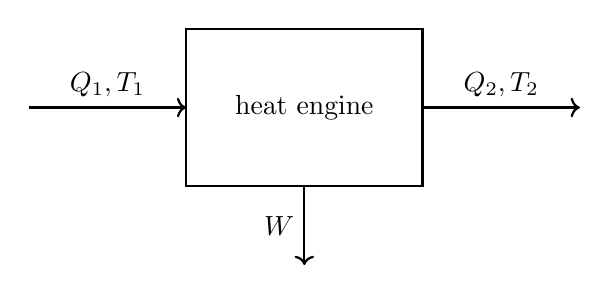
\begin{tikzpicture}
        \draw[thick] (0,0) rectangle (3,2) node[midway] {heat engine};
        
        \draw[->, thick] (-2,1) -- (0,1) node[midway, above] {$Q_1, T_1$};
        \draw[->, thick] (3,1) -- (5,1) node[midway, above] {$Q_2, T_2$};
        \draw[->, thick] (1.5,0) -- (1.5,-1) node[midway, left] {$W$};
    \end{tikzpicture}
\end{center}
energy balance:
\[ \cancel{\frac{dU}{dt}} = \dot{Q} + \dot{W_s} + \cancel{\sum \dot{m}_k()_k} \]
\[ 0 = Q_1 + Q_2 + W\]
entropy balance:
\[ \cancel{\frac{dS}{dt}} = \frac{\dot{Q}_1}{T_1} + \frac{\dot{Q}_2}{T_2} + \cancel{\sum_{k=1}^{K}\dot{m}_k \hat{S}_k} + \dot{S}_{\text{gen}} \]
\[ 0 = \frac{\dot{Q}_1}{T_1} + \frac{\dot{Q}_2}{T_2}  + \dot{S}_{\text{gen}} \]
integrating, and remembering that reversible processes are more efficient than irreversible processes
\[ 0 = \frac{Q_1}{T_1} + \frac{Q_2}{T_2} \]
\[ \frac{Q_1}{T_1} = \frac{- Q_2}{T_2} \]
\[ Q_2 = \frac{- Q_1 T_2}{T_1} \]
and taking this into the energy balance
\[ -W_s= Q_1 + \frac{- Q_1 T_2}{T_1} = Q_1 \left(\frac{T_1 - T_2}{T_1}\right) \]
\[ \eta = \frac{-W_s}{Q_1} = \left(\frac{T_1 - T_2}{T_1}\right) \]
\subsection*{back to the actual problem}

\noindent
Let the system be the block (the yellow thingy). The energy balance in difference form simplified (please don't crucify me for skipping to simplified balances)
\[ \Delta U = Q_H \]
\[ dU = dQ_H \]
\[ \frac{dU}{dT_H} = C_v \]
\[ dU = C_v dT_H \]
Now for the carnot engine we know this relationship will hold
\[ \frac{-W_S}{Q_H} = 1 - \frac{T_c}{T_H} \]
which, in terms of infinitecimals
\[ \frac{-dW_s}{dQ_h} = 1 - \frac{T_c}{T_H} \]
\[ -dW_s = dQ_h \left[1 - \frac{T_c}{T_H}\right] \]
and applying the result of the energy balance
\[ -dW_s = C_v dT+H \left[1 - \frac{T_c}{T_H}\right] \]
now integrating to sum up all the dQ
\[ -W_s = \int_{T_1}^{T_2} C_v dT_H - \int_{T_1}^{T_2}C_v \frac{T_c}{T_H} dT_H \]
\[ -W_s = C_v \left(T_2 - T_1\right) - C_v T_c \ln \left(\frac{T_2}{T_1}\right) \]
and just turning the absolute heat capacity into a not so absolute heat capacity
\[ -W_s = m\hat{C}_v \left(T_2 - T_1\right) - m\hat{C}_v T_c \ln \left(\frac{T_2}{T_1}\right) \]
which now may be used to calculate out the two different exergies and compare them

\begin{table}[H]
\centering
\begin{tabular}{ccc}
    \toprule
    Parameter & Case 1 & Case 2 \\
    \midrule
    $T_H$ & 500 K & 400 K \\
    $T_C$ & 300 K & 300 K \\
    $m$ & 100 kg & 200 kg \\
    $\hat{C_p}$ & 500 J/kg K & 500 J/kg K \\
    $-W_S$ & 2.33 MJ & 1.37 MJ \\
    \bottomrule
\end{tabular}
\end{table}
\boxed{\text{The block that starts at 500 K has more exergy.}}




\section*{3.}
\begin{center}
    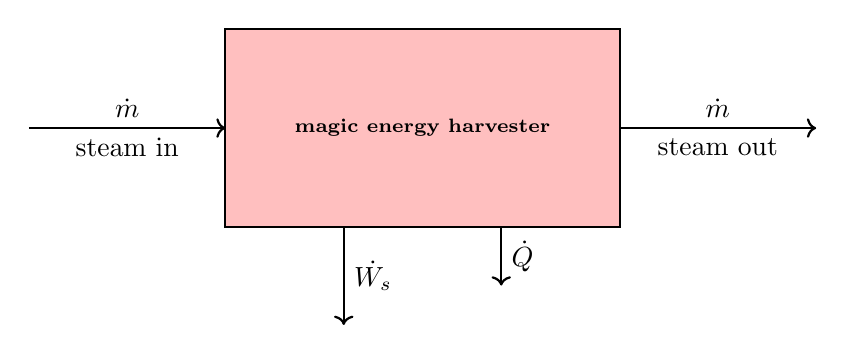
\begin{tikzpicture}
        \draw [->, thick] (0.0, 9.5) -- (2.5, 9.5) node[midway, above]{$\dot{m}$} node[midway, below]{steam in};
        \draw [->, thick] (7.5, 9.5) -- (10.0, 9.5) node[midway, above]{$\dot{m}$} node[midway, below]{steam out};
        \draw [->, thick] (4, 8.25) -- (4, 7.) node[midway, right]{$\dot{W_s}$};
        \draw [->, thick] (6, 8.25) -- (6, 7.5) node[midway, right]{$\dot{Q}$};
        \draw[line width=0.5mm] (2.5, 10.75) rectangle (7.5, 8.25);
        \fill[pink] (2.5, 10.75) rectangle (7.5, 8.25);
        \node at (5.0, 9.5) {\bfseries\scriptsize magic energy harvester};
    \end{tikzpicture} % $\dot{Q}$
\end{center}
the system is the carnot engine. this system is at steady state. the mass balance is
\[ \frac{dm}{dt} = 0 \rightarrow \dot{m}_{in}  = \dot{m}_{out} = \dot{m} \]
energy balance
\[ 0 = \dot{Q} + \dot{W}_s + \sum_{k=1}^{K}\dot{m}_k \hat{H}_k = \dot{Q} + \dot{W}_s + \dot{m}\left(\hat{H}_{in} - \hat{H}_{out}\right) \]
entropy balance
\[ 0 = \dot{m}\left(\hat{S}_{in} - \hat{S}_{out}\right) + \frac{Q}{T} + \dot{S}_{gen} \]
but a reversible process is more efficient than an irreversible process, so, 
\[ 0 = \dot{m}\left(\hat{S}_{in} - \hat{S}_{out}\right) + \frac{Q}{T}  \]
and rearranging the entropy balance and slap---smacking it into the energy balance
\[ \dot{Q} = T_{out} \dot{m} \left( \hat{S}_{out} - \hat{S}_{in} \right) \]
\[ \dot{m}\left[\left(\hat{H}_{in} - T_{out}\hat{S}_{in}\right) - \left(\hat{H}_{out} - T_{out}\hat{S}_{out}\right)\right] + W_s = 0 \]
\[ -W_s = \dot{m}\left[\left(\hat{H}_{in} - T_{out}\hat{S}_{in}\right) - \left(\hat{H}_{out} - T_{out}\hat{S}_{out}\right)\right]  \]
now going into the depths of the steam tables to look up the enthalpys and entropys
\begin{itemize}
    \item $\hat{H}$ (200C, 1 bar) = 2875.3
    \item $\hat{H}$ (25C, 1 bar) = 104.89
    \item $\hat{S}$ (200C, 1 bar) = 7.8343
    \item $\hat{H}$ (25C, 1 bar) = 0.3674
\end{itemize}
also converting the flow rate
\[ 3.6\,\frac{\text{tons}}{\text{hr}} \times \frac{1000\,\text{kg}}{1\,\text{ton}} \times \frac{1\,\text{hr}}{3600\,\text{sec}} = 1.0\,\text{kg/s} \]
plugging everything into the derived equation
\begin{align*}
    -W_s &= 1 \left(2875.3 - 298 \times 7.8343 - \left(104.89 - 298 \times 0.3674\right)\right) \\
    -W_s &= 545.3\,\text{kJ/s}
\end{align*}



\section*{4.}
To tell if a process is thermodynamically possible it needs to satisfy all the equations and it needs to have non--negative $\dot{S}_{gen}$. Let's take a look at this hilsch tube I've been hearing about\dots
\begin{center}
    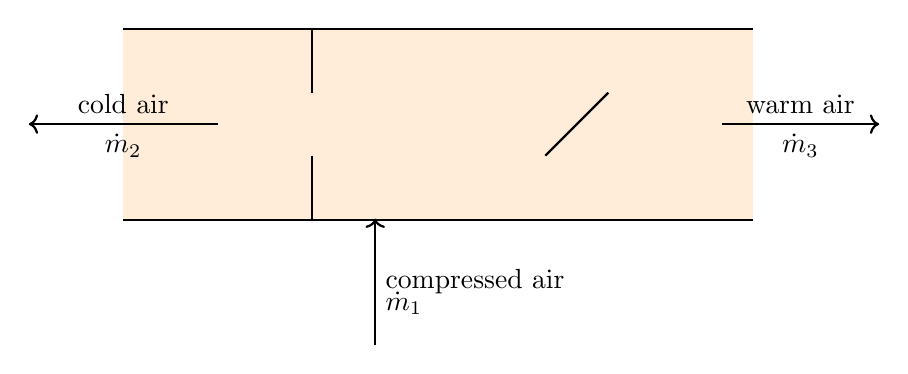
\begin{tikzpicture}[scale=0.8]
        \draw[thick, line width = 0.5mm] (2.5, 9.65) -- (12.5, 9.65);
        \draw[thick, line width = 0.5mm] (2.5, 6.65) -- (12.5, 6.65);
        \fill[orange!15!white] (2.5, 9.65) rectangle (12.5, 6.65);
        \draw[thick] (5.5, 9.65) -- (5.5, 8.65);
        \draw[thick] (5.5, 7.65) -- (5.5, 6.65);
        \draw[thick] (9.2, 7.65) -- (10.2, 8.65);
        \draw[thick, ->] (4.0, 8.15) -- (1.0, 8.15) node[midway, above]{cold air} node[midway, below]{$\dot{m}_2$};
        \draw[thick, ->] (12.0, 8.15) -- (14.5, 8.15)node[midway, above]{warm air} node[midway, below]{$\dot{m}_3$};;
        \draw[thick, ->] (6.5, 4.65) -- (6.5, 6.65)node[midway, right]{compressed air} node[midway, below right]{$\dot{m}_1$};;
    \end{tikzpicture}
\end{center}
the mass balance looks like
\[ 0 = \dot{n}_{1} - \dot{n}_{2} - \dot{n}_{3}  \]
and we know mass in = mass out and that its a 50--50 split
\[ \dot{n}_1 = 2 \dot{n}_2 = 2 \dot{n}_3 = \dot{n} \]
energy balance
\[ 0 = \dot{n}_{1} \ub{H}_1 - \dot{n}_{2} \ub{H}_2 - \dot{n}_{3} \ub{H}_3 \]
\[ 0 = 2 \ub{H}_1 -  \ub{H}_2 -  \ub{H}_3 \]
\[ 0 =  \left(\ub{H}_1 -  \ub{H}_2\right) + \left(\ub{H}_1 -  \ub{H}_3\right) \]
and remembering that $\Delta \ub{H} = {C}_p^* \Delta T$ for constant $C_p^*$
\[ 0 = \hat{C}_p \left(T_1 - T_2\right) + \hat{C}_p \left(T_1 - T_3\right) \]
\[ 0 =  \left(T_1 - T_2\right) +  \left(T_1 - T_3\right) \]
\[ T_1 = \frac{1}{2} \left(T_2 + T_3\right) = 300\,\text{K} \]
now we toss this into the entropy balance to see if $\dot{S}_{gen}>0$
\[ 0 = \sum n_k \ub{S}_k  + \dot{S}_{gen} = n\left( \ub{S}_1 + \frac{1}{2}\ub{S}_2 + \frac{1}{2} \ub{S}_3 \right) + \dot{S}_{gen} \]
\[ 0 = \frac{1}{2}n \left(\left(\ub{S}_1 - \ub{S}_2\right) + \left(\ub{S}_1 - \ub{S}_3\right)\right) + \dot{S}_{gen} \]
and now using that silly ideal gas adiabatic change in entropy equation derived from the gibbs equation
\[ -\dot{S}_{gen} = \frac{1}{2}n\left(\left(C_p \ln\left(\frac{T_2}{T_1}\right) - R \ln \left(\frac{P_2}{P_1}\right)\right) +\left(C_p \ln\left(\frac{T_3}{T_1}\right) - R \ln \left(\frac{P_3}{P_1}\right)\right) \right) \]
\[ \dot{S}_{gen} = -\frac{1}{2}n\left(\left(35.026 \ln\left(\frac{100}{300}\right) - 8.3145 \ln \left(\frac{1}{3.33}\right)\right) +\left(35.026 \ln\left(\frac{500}{300}\right) - 8.3145 \ln \left(\frac{1}{3.33}\right)\right) \right) \]
\[ \dot{S}_{gen} = -0.292n \]
since the entropy generation is negative, this process is impossible.




\section*{5.}
Assume air is a diatomic gas in ideal state s.t. $C_p = \frac{7}{2} R$ and $C_v = \frac{5}{2} R$. 
\subsection*{a. adiabatic, reversible turbine}
\begin{center}
    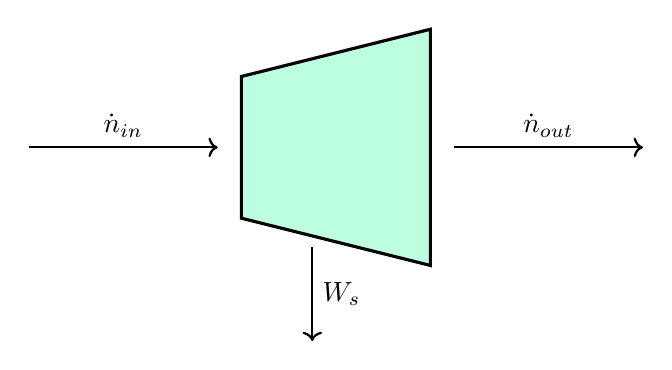
\begin{tikzpicture}[scale=1.2]
        \draw [->, thick]  (2.0, 9.15) -- (4.0, 9.15) node[midway, above]{$\dot{n}_{in}$};
        \draw [->, thick]  (5.0, 8.1) -- (5.0, 7.1) node[midway, right]{$W_s$};
        \draw [->, thick]  (6.5, 9.15) -- (8.5, 9.15) node[midway, above]{$\dot{n}_{out}$};
        \draw [line width=0.4mm, fill={rgb,255:red,188;green,255;blue,224}] (6.25, 10.4) -- (6.25, 7.9) -- (4.25, 8.4) -- (4.25, 9.9) -- cycle;
    \end{tikzpicture}
\end{center}
Let the system be the contents of the turbine highlighted in mint green. Mass balance:
\[ 0 = \dot{n}_{in} - \dot{n}_{out} \]
energy balance
\[ 0 = -\dot{W_s} + \dot{n}_{in}\hat{H}_{in} - \dot{n}_{out}\hat{H}_{out} \]
\[ -W_s = \dot{n}\left(\hat{H}_{out} - \hat{H}_{in}\right) \]
entropy balance
\[ 0 = \dot{n}\left(\ub{S}_{in} - \ub{S}_{out}\right) \] \marginpar{isentropic!}
\[ \ub{S}_{in} = \ub{S}_{out} \] 
now bringing in that one fun equation derived from the gibbs equation
\[ \Delta \ub{S} = 0 = C_p \ln \left(\frac{T_2}{T_1}\right) - R \ln\left(\frac{P_2}{P_1}\right) \]
\[ \left(\frac{T_2}{T_1}\right)^{C_p} = \left(\frac{P_2}{P_1}\right)^{R} \]
\[ T_2 = T_1 \left(\frac{P_2}{P_1}\right)^{R/C_p} \]
\[ T_2 = 400 \left(\frac{1.01325}{10}\right)^{8.3145/(3.5 * 8.3145)} \]
\[ T_2 = 208\,\text{K}\]
remembering $\Delta H = C_p \Delta T$ for constant $C_p$
\[ -W_s = \dot{n}C_p\left(T_{out} - T_{in}\right) \]
and now because this question is annoyingly ideal i'll use the ideal gas law to find the molar volume
\[ \ub{V} = \frac{RT}{P} = \frac{8.3145 \times 400}{10 \times 10^{5}} \times 1000\frac{\text{L}}{\text{m}^2} = 3.33 \frac{\text{L}}{\text{mol}} \]
\[ \dot{n} = \frac{10\,\text{L/s}}{3.33\,\text{L/mol}} = 3.01\,\text{mol/s} \]
back to the equation from the energy and mass balance
\begin{align*}
    -\dot{W}_s &= 3.01 \times 29 \left(400 - 208\right) \\
    -\dot{W}_s &= 16782\,\text{kJ/s}
\end{align*}




\subsection*{b. isothermal turbine}
\begin{center}
    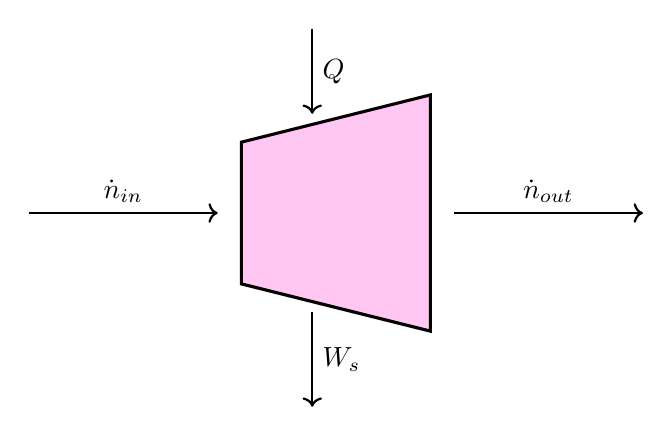
\begin{tikzpicture}[scale=1.2]
        \draw [->, thick]  (2.0, 9.15) -- (4.0, 9.15) node[midway, above]{$\dot{n}_{in}$};
        \draw [->, thick]  (5.0, 8.1) -- (5.0, 7.1) node[midway, right]{$W_s$};
        \draw [->, thick]  (5.0, 11.1) -- (5.0, 10.2) node[midway, right]{$Q$};
        \draw [->, thick]  (6.5, 9.15) -- (8.5, 9.15) node[midway, above]{$\dot{n}_{out}$};
        \draw [line width=0.4mm, fill={rgb,255:red,255;green,198;blue,241}] (6.25, 10.4) -- (6.25, 7.9) -- (4.25, 8.4) -- (4.25, 9.9) -- cycle;
    \end{tikzpicture}
\end{center}
mass balance
\[ \dot{m}_{in} = \dot{m}_{out} = \dot{m} \]
energy balance
\[  0 = W_s + Q - m\left(\hat{H}_{out} - \hat{H}_{in}\right)  \]
however, we know that for an ideal gas the enthalpy is only a function of temperature so $\Delta H = 0$ 
\[  -W_s = Q  \]
now looking at the entropy balance {\scriptsize differential flavor}
\[ 0 = \frac{\dot{Q}}{T} + \dot{n}\left(\ub{S}_{in} - \ub{S}_{out}\right) + \highlight{red}{\dot{S}_{gen}} \]
since the problem statement said 100\% efficient, no entropy is generated
\[ 0 = \frac{\dot{Q}}{T} + \dot{n}\left(\ub{S}_{in} - \ub{S}_{out}\right)  \]
\[ \dot{Q} = T \dot{n} \left(\ub{S}_{out} - \ub{S}_{in}\right) \]
remembering the $\Delta S$ equation that comes from the gibbs equation
\begin{align*}
    \Delta \ub{S} &= C_p \ln\left(\frac{T_2}{T_1}\right) - R \ln\left(\frac{P_2}{P_1}\right) \\
     &= - R \ln\left(\frac{P_2}{P_1}\right) \\
     &= - R \ln\left(\frac{1.01325\,\text{bar}}{10\,\text{bar}}\right) \\
    &= 19.04 \frac{\text{kJ}}{\text{mol}\cdot\text{K}}
\end{align*}
and going back to the energy balance
\[ -W_s = Q = T \dot{n} \Delta \ub{S} = 400 \times 3 \times 19.04 = 22865\,\text{kJ/s} \]



\subsection*{c. maximum theoretical}
% {\Huge do this one later, still on ipad needing to get finished}
% \begin{center}
%     \begin{tikzpicture}[scale=0.7]
%         \draw [line width=0.5mm, fill={rgb,255:red,255;green,255;blue,255}] (8.0, 10.85) circle (1.5);
%         \draw [->, thick] (2.5, 10.85) -- (6.0, 10.85) node[midway, above]{steam in};
%         \draw [->, thick]  (10.0, 10.85) -- (13.5, 10.85) node[midway, above]{steam out};
%         \draw [->, thick]   (8.0, 8.95) -- (8.0, 6.55) node[midway, right]{$Q_H$};
%         \draw [->, thick]   (11.5, 5.35) -- (13.5, 5.35) node[midway, above]{$Q_c$};
%         \draw [thick]   (8.0, 4.35) -- (8.0, 3.35);
%         \draw [->, thick]   (8.0, 3.35) -- (13.5, 3.35) node[midway, above]{$W_s$};
%         \draw [thick]   (5.5, 9.35) -- (7.5, 11.35);
%         \draw [thick]   (7.5, 11.35) -- (8.5, 10.35);
%         \draw [->, thick]   (8.5, 10.35) -- (10.5, 12.35);
%         \draw [line width=0.5mm, fill={rgb,255:red,255;green,255;blue,255}] (5.0, 6.35) rectangle (11.5, 4.35);
%         \node at (8.25, 5.35) {Carnot Engine};
%     \end{tikzpicture}
% \end{center}
% Let the system be the entire depicted apparatus consisting of a heat exchanger and a carnot engine. the mass balance is straight forward (system is at steady state)
% \[ \frac{dm}{dt} = 0 \longrightarrow \dot{m}_{in} = \dot{m}_{out} = \dot{m} \]
% energy balance letting the system be the carnot engine
% \[ 0 = W_s + Q +  \]
consider the steam going through a magical black box that extracts all the energy from the steam until it is in the dead state.
\begin{center}
    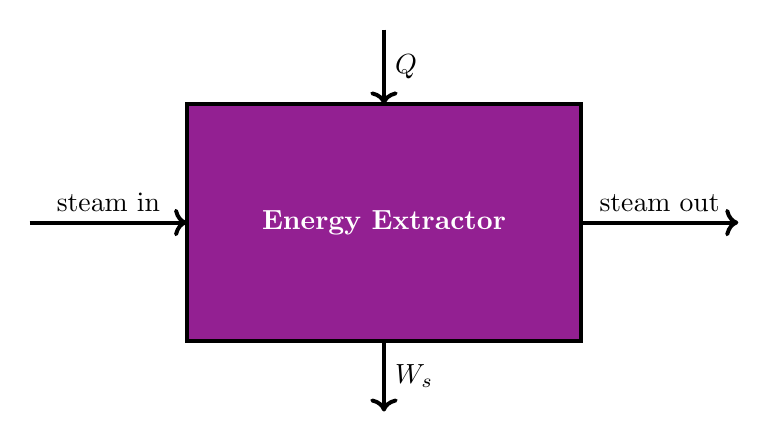
\begin{tikzpicture}
        \draw [->, line width=0.5mm] (0.5, 7.65) -- (2.5, 7.65) node[midway,above]{steam in};
        \draw [->, line width=0.5mm] (7.5, 7.65) -- (9.5, 7.65) node[midway,above]{steam out};
        \draw [->, line width=0.5mm] (5.0, 6.15) -- (5.0, 5.25) node[midway,right]{$W_s$};
        \draw [->, line width=0.5mm] (5.0, 10.1) -- (5.0, 9.15) node[midway,right]{$Q$};
        \draw [line width=0.5mm, fill={rgb,255:red,147;green,32;blue,146}] (2.5, 9.15) rectangle (7.5, 6.15);
        \node [white] at (5.0, 7.65) {\bfseries Energy Extractor};
    \end{tikzpicture}
\end{center}
the system is the contents of the energy extractor. mass balance
\[ \frac{dn}{dt} = 0 = \dot{n}_{in} - \dot{n}_{out} \]
\[ \dot{n}_{in} = \dot{n}_{out} = \dot{n} \]
energy balance
\[ \frac{dU}{dt} = 0 = W_s + Q + \dot{n}_{in}\ub{H}_{in} - \dot{n}_{out}\ub{H}_{out} \]
entropy balance, noting that reversible processes are more efficient than irreversible processes
\[ \frac{dS}{dt} = 0 = \dot{n}_{in}\ub{S}_{in} - \dot{n}_{out}\ub{S}_{out} + \frac{Q}{T_{\text{ambient}}} \]
\[ \dot{Q} = \dot{n}\left(\ub{S}_{out} - \ub{S}_{in}\right) \]
now substituting that into the energy balance
\[ 0 = W_s + \dot{n}\left(\ub{S}_{out} - \ub{S}_{in}\right) +\dot{n}\ub{H}_{in} - \dot{n}_{out}\ub{H}_{out} \]
\[ -W_s = \dot{n} \left[ \left(\ub{H}_{in} - T_{\text{ambient}}\ub{S}_{in}\right) - \left(\ub{H}_{out} - T_{\text{ambient}}\ub{S}_{out}\right) \right] \]
\[ -W_s = \dot{n} \left[ \left(\ub{H}_{in} - \ub{H}_{out}\right) - T_{\text{ambient}}\left(\ub{S}_{in} - \ub{S}_{out}\right) \right] \]
\marginpar{both $\Delta$}
\marginpar{are negative}
\[ -W_s = \dot{n} \left[ \left(- C_p^* \Delta T \right) + T_{\text{ambient}}\left(C_p^* \ln \left(\frac{T_2}{T_1}\right) - R \ln \left(\frac{P_2}{P_1}\right)\right) \right] \]
\[ -W_s = 3 \left[ \left( (29) (400-298) \right) + 298\left(29 \ln \left(\frac{298}{400}\right) - 8.3145 \ln \left(\frac{1.013}{10}\right)\right) \right] \]
\[ -W_s = 18266\,\text{kW} \]




\section*{6.}

\subsection*{a.}
\centmini{0.8}{
    \subsubsection*{a.}
    \[ d\ub{U} = \p{\ub{U}}{\ub{S}}{\ub{V}} d\ub{S} + \p{\ub{U}}{\ub{V}}{\ub{S}} d\ub{V} \]
    \subsubsection*{b.}
    \[ d\ub{H} = \p{\ub{H}}{\ub{S}}{P} d\ub{S} + \p{\ub{H}}{P}{\ub{S}} dP \]
    \subsubsection*{c.}
    \[ d\ub{H} = \p{\ub{H}}{T}{P} dT + \p{\ub{H}}{P}{T} dP \]
}

\subsection*{b.}
restating the fundemental relationship
\[ d\ub{U} = T d\ub{S} - P d\ub{V} \] 
and now turning this into a complete/total differential
\[ d\ub{U} = \p{\ub{U}}{\ub{S}}{\ub{V}} d\ub{S} - \p{\ub{U}}{\ub{V}}{\ub{S}} d\ub{V} \]
we see this
\[ d\ub{U} = \highlight{red}{T} d\ub{S} \highlight{blue}{- P} d\ub{V} \]
\[ d\ub{U} = \highlight{red}{\p{\ub{U}}{\ub{S}}{\ub{V}}} d\ub{S} - \highlight{blue}{\p{\ub{U}}{\ub{V}}{\ub{S}}} d\ub{V} \]
so now just putting this as an equation so it feels all formalized
\[ \p{\ub{U}}{\ub{S}}{\ub{V}} = T \]
\[ \p{\ub{U}}{\ub{V}}{\ub{S}} = - P \]






\section*{7.}
Starting off by writing the total differential
\[ d\ub{H} = \p{\ub{H}}{T}{P} dT + \p{\ub{H}}{P}{T} dP \]
\[ \pop{T}{\ub{H}} d\ub{H} = \highlight{red}{\p{\ub{H}}{T}{\ub{H}}}  = \p{\ub{H}}{T}{P} \highlight{green}{\p{T}{T}{\ub{H}}} + \p{\ub{H}}{P}{T} \p{P}{T}{\ub{H}} \]
remembering the rules tells us that the red term is 0 and the green term is 1
\[0 = \p{\ub{H}}{T}{P} + \p{\ub{H}}{P}{T} \p{P}{T}{\ub{H}} \]
\[ \p{\ub{H}}{T}{P} = - \p{\ub{H}}{P}{T} \p{P}{T}{\ub{H}}  \]
and now diving over the ones on the right since we can do that thanks to rule 3
\[ \p{\ub{H}}{T}{P} \p{P}{\ub{H}}{T} \p{T}{P}{\ub{H}} = - 1  \]









\end{document}